\documentclass[a4paper, openany]{memoir}

\usepackage[utf8]{inputenc}
\usepackage[T1]{fontenc} 
\usepackage[english]{babel}
\usepackage{amsmath}
\usepackage{amssymb}

\usepackage{booktabs}
\usepackage{fancyhdr}
\usepackage{float}
\usepackage{indentfirst}
\usepackage{graphicx}
\usepackage[linewidth=1pt]{mdframed}
\usepackage{multicol}
\usepackage{fancyvrb}

\pagestyle{fancy}
\fancyhf{}
\fancyhead[LE]{\leftmark}
\fancyhead[RO]{\rightmark}
\fancyhead[RE, LO]{PSD}
\fancyfoot[LE, RO]{\thepage}
\fancyfoot[RE, LO]{Pete Gautam}

\renewcommand{\headrulewidth}{1.5pt}

\chapterstyle{thatcher}
\setcounter{chapter}{6}

\begin{document}

\chapter{Code Reviews}
Code reviews are an important and a very popular software quality assurance practice. It complements other techniques, such as testing. In this section, we will look at source code review practices, but it is also possible to review:
\begin{itemize}
    \item source code documentation (inline comments and high-level documentation, e.g. design documentation)
    \item test code
    \item design descriptions
    \item requirements specifications, i.e. what the system should do.
\end{itemize}
Essentially, any configuration item in a version control repository can be subject of review. Artifacts not controlled in this way should not be reviewed. This is because it is not possible to track the consequences of change recommendations to the artifact.

There are many reasons to undertake a code review. The historical reason for doing so is to detect defects in the software. In modern practice, there are many more reasons to do so, including:
\begin{itemize}
    \item to identify refactoring opportunities of poorly structured code.
    \item to develop a shared understanding of code between developers. In particular, it can allow novice developers to conduct a review for code submitted by experts, or vice versa.
    \item to share good practices between team members, e.g. the reviewer may recommend to use some design pattern.
    \item to gain knowledge about legacy systems, e.g. when looking at a poorly documented code base and improving it. This is done to gain a wider understanding about how the software functions. In this case, we are not trying to improve the quality of the software. Instead, we are distributing knowledge between the team.
\end{itemize}
So, there are a wide variety of purposes for code reviews. These help share understanding and foster collective ownership of code between the developers. It is an opportunity for the source code to be improved collaboratively.

Code reviews should not be used for performance evaluation. This would incentivise the delivery of a higher quality software. The developers will try to gain approval among the team and submit a better quality code in the first place. They will also want to submit proposed changes that are easier for their reviewers to perform a review on. 

So, it can be tempting to introduce incentivisation into the process, e.g. bonus for good submissions and penalty for bad submissions. This is extremely risky. It changes focus of the code review from collaborative improvement of code and sharing of knowledge to performance evaluation of the team member. This can create tension and conflict between the members. This is because they are being reviewed by each other in a way that could affect their future.

Historically, code reviews took place periodically. A portion of the accepted code base was selected for inspection before release, in order to detect any defects and to recommend any removal. It was common to choose the portion depending on the most changed section of the code, or the section where there is a higher likelihood of bugs to be present.

Nowadays, code reviews take place on a proposed change to the code base, after a merge request and before its approval. In the case of a legacy system, we perform code reviews before a proposed change so that we can understand a portion of the code base before attempting to make a change.

Now, we consider whether code reviews work. We define the total defects to be:
\[\text{total defects} = \text{undetected defects} \cup \bigcup_{m \in \text{methods}} \text{defects}(m).\]
That is, the set of all the defects is composed of undetected defects and defects that have been found by some quality-assurance method. Undetected defects are those that get reported after the release, by some user. Using this, we can compute the defect detection rate for a method $m$:
\[\text{defect detection rate}(m) = |\text{defects}(m)|/|\text{total defects}|.\]
Now, we consider the defect detection rate for code reviews in multiple papers:
\begin{itemize}
    \item Fagan (1976) reported the defect detection rate about about 66-82\% for 2 studies that used comprehensive inspection process.
    \item Jones (1986) reported the defect rate of 60\% for design inspections alone, and 25\% for unit testing.
    \item Boehm (1981) reported that inspections (in 4 case studies) uncovered between 63\% and 75\% of the defects.
    \item Wilkerson et al (2012) reported that fewer defects were left in a software using code reviews than using test-driven development.
    \item Runseon et al (2006) reported that the effectiveness of code reviews and inspections was linked to the nature of the software under inspection.
\end{itemize}

\section{Workflow of code reviews}
The following image summarises the workflow of code reviews:
\begin{figure}[H]
    \centering
    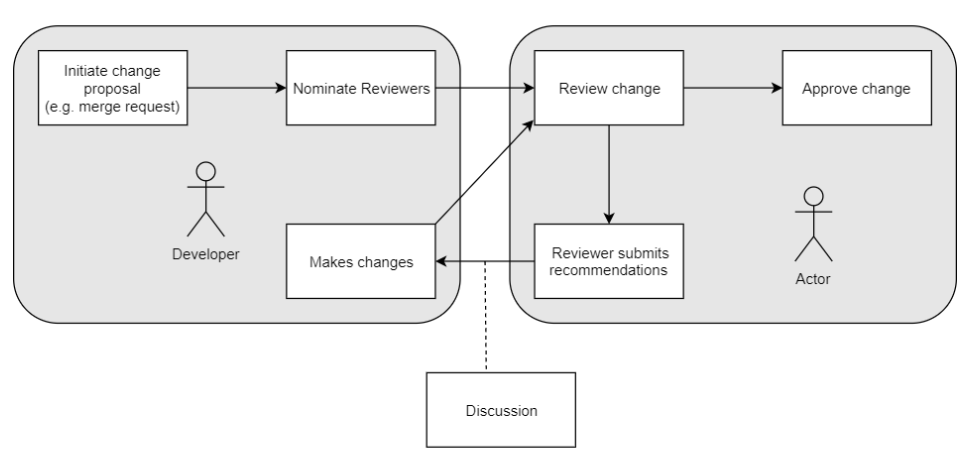
\includegraphics[scale=0.5]{src/7 code reviews workflow.PNG}
\end{figure}
First, the developer proposes change (e.g. via a merge request from one branch to another). The nature of the source branch depends on the type of the project. Small teams maintain development branches in the same repository as the master branch. In open-source projects, it is more common for a developer to fork the entire repository and make a pull request of the forked repository back to the master branch. 

The developer will select reviewers from the development team. The team might have guidelines for who is appropriate to review the code depending on the type of change. Moreover, modern tools recommend reviewers based on different policies, e.g. based on the files that have been changed in the pull/merge request, and the developer who frequently updated these files.

Many teams assume that the reviewer should be as experience as the submitting developer. But, there are benefits to choosing a junior colleague for code reviews. It can help with the shared understanding of code and can elicit new approaches to structuring code. Junior developers have good ideas as well as experienced colleagues.

Reviewers then annotate the merge request with recommended changes. These recommendations are returned back to the developer for consideration. The developer might then make a number of changes and resubmit code for further review (with perhaps a different reviewer). 

During this process, it is very important and useful for the developer and the reviewer to discuss and follow up on any recommendations that the reviewer has made. This can help clarify why the recommendation was made and what the reviewer is trying to achieve with the developer. 

This process occurs several times until the proposed change is accepted by reviewers. Then, the changes get approved, and the developer merges the code into the master branch.

\section{Good practices for merge requests}
A single review should be at most about 300 lines of code. If it is higher, the review process takes longer, which slows down the returned feedback. Moreover, the reviewer is more likely to miss defects. It should be possible to complete a review within about 30 minutes, including making the recommendations. A large merge request should be broken into smaller change packages. The team should incorporate the code review time into their workload model. It is part of the project's estimate of work efforts to conduct these reviews.

When describing the change request, it is important to identify a single purpose. Typically, the purpose is one of the following:
\begin{itemize}
    \item Corrective- the change resolves bugs and so the description should refer to the bug explicitly. In particular, it should summarise the defective behaviour and the correct behaviour that has been realised by the change.
    \item Adaptive- the change is a response to changes in the system's environment, e.g. the team needs to migrate to a new release of the dependency/language implementation.
    \item Perfective- the change adds new features to the system. The description should state what the new feature does, and refer to the requirement specification.
    \item Preventative- the change enhances maintainability of the code, e.g. by refactoring it.
\end{itemize}

Requiring the developer to pick a single purpose for a change can be helpful in communicating the rationale of the change to the reviewers. If a change has multiple purposes, it should be broken into smaller chunks where each chunk has a single purpose. Once a single purpose is identified, the developer can give the change request a succinct title and a description to explain its purpose. 

It is also good for the developer to talk about wider impacts of the change, e.g. the code makes breaking changes to an API for the software, or it removes some functionality for the end user. The developer can include specific aspects of change that they are seeking feedback for, e.g. they might know that the code isn't optimal, so they want expert feedback on optimising it.

\section{CI and code reviews}
Code reviews are expensive, so we should use automation to remove as many issues as possible before a merge request (and code review). The review should focus on subjective judgments that cannot be automatically eliminated. A CI tool can be configured so that changes cannot be applied on master until a wide range of automated tests pass. For example, if a change request is too large (e.g. more than 300 lines of code), then the merge request should be rejected by the CI tool. A change request might also be blocked if:
\begin{itemize}
    \item the change breaks tests;
    \item the change violates the code style;
    \item there is commented out code;
    \item there are spelling mistakes in the identifier;
    \item the test coverage gets reduced.
\end{itemize}

Static and dynamic analysis can be useful to locate smells and help prioritise code reviews and focus efforts. We can use source code metrics such as the number of liens of code per function, and the number of executable per the number of the comment lines. The latter can indicate where large amounts of comments are being used for poorly structured code. We can also find out if there are large method bodies included in the code base.

Design metrics (e.g. cyclometric complexity) are useful for identifying poorly structured modules which are amenable to refactoring. 

Test suite metrics address effectiveness and efficiency of test suite, e.g. test suite coverage and mutation testing. These can be used to avoid having a change reduce the effectiveness of test suites.

Usage pattern analysis can defect memory and I/O leaks or typecast errors. It can prevent performance defects. It helps spot potential smells that might include defects. 

It is a good idea to use a merge conflict template to ensure consistent style within the repository. It can help merge review process by having a common template shared across the team.

\section{Code review questions}
During the review, the following are some questions that the reviewer can ask:
\begin{itemize}
    % purpose
    \item Does this change solve the problem? Is the problem clearly stated?
    \item How would I solve the problem? What would I have done differently? This can be useful in identifying better patterns of implementation to solve the problem.
    \item Has dependent documentation, e.g. user guides, been updated alongside the change in the implementation of the functional behaviour?
    % quality assurance
    \item What are the typical and extreme use cases for this code? Are they covered by test cases?
    \item Has the developer thought of corner cases (e.g. empty collections, parameter boundaries), e.g. is the value of an integer assumed to be positive?
    \item How does the code handle exceptional situations, e.g. when there is a loss of internet connectivity, if a file is missing, etc.
    % architecture
    \item Does the change follow the existing architectural conventions for the software? A team develops a culture/style within the system, e.g. developing functionality through a plugin architecture. Has the developer been consistent and followed the team's architectural conventions?
    \item Are there missed opportunities for reuse of existing code? The developer might have re-implemented a functionality within the solution that already exists within the production code/the standard libraries in the framework being used.
    \item Are there clones present in the change? A clone is a duplicate sequence of statements within a change. It might be possible to extract those changes and make them abstract, hence refactoring the code base.
    % code
    \item Do identifiers follow suitable naming conventions? Is their purpose self-evident? Using an abbreviation might make it less clear.
    \item Is the code self-documenting? Can I (easily) understand what the code is supposed to do without the need of comments.
    \item Are all the source code comments necessary? Source code comments should explain why a particular implemented has been adopted, and not how. Excessive documentation might mean that the solution is poorly implemented.
    \item Are comments necessary to describe why a particular implementation has been chosen? For example, when using an API, we may need to implement a functionality in a particular way that is not intuitive. Source code comments can be used to explain this method.
    % non-functional requirements
    \item Are performance optimisations possible? For example, has the developer searched the entire set if only a small subset needs to be considered?
    \item Are efficiency optimisations possible?
    \item Are relevant security patterns followed? Has the developer introduced a vulnerability in their proposed change?
\end{itemize}

\section{Real-time code reviews}
There are 2 alternatives to code reviews- pair programming and mob programming. In pair programming, 2 developers work together to implement code. One of them is the driver, who types the code. The other one is the navigator. They pass instructions to the driver, and do not code directly. This is effectively real-time code review as the two developers are working together and reviewing each other's code as it is being created. In mob programming, an entire team works collectively in implementing a single solution in a similar way to pair programming.

In summary, code reviews should be considered a collaborative approach to improving the quality of the software system. Historically, this involved identifying recommendations to remove defects. But, nowadays, there are far wider benefits in code reviews in terms of collaborative improvement of code.


\end{document}